
%%%%%%%%%%%%%%%%%%%%%%%%%%%%%%%%%%%%%%%%%%%%%%%%%%%%%%%%%%%
\section{Experiment}\label{sec:expResults}
%%%%%%%%%%%%%%%%%%%%%%%%%%%%%%%%%%%%%%%%%%%%%%%%%%%%%%%%%%%



%\subsection{Hardware System}


Our experiments are on centimeter-scale hardware systems called \emph{kilobots}.  These allows us to emulate a variety of dynamics, while enabling a high degree of control over robot function, the environment, and data collection. The kilobot, from \cite{Rubenstein2012,rubenstein2014programmable} is a low-cost robot designed for testing collective algorithms with large numbers of robots. It is available as an open source platform or commercially from~\cite{K-Team2015}.  Each robot is approximately 3 cm in diameter, 3 cm tall, and uses two vibration motors to move on a flat surface at speeds up to 1 cm/s.  Each robot has one ambient light sensor that is used to implement \emph{phototaxis},  moving towards a light source. 
In these experiments as shown in Fig.~\ref{fig:setup}, we used $n$=97 kilobots, a glass-covered 1.5 m$\times$1.2 m whiteboard as the workspace, and eight 30W LED floodlights arranged 1.5 m above the plane of the table at the $\{N,NE,E,SE,S,SW,W,NW\}$ vertices of a 6 m square centered on the workspace. The lights were controlled using an Arduino Uno board connected to an 8-relay shield.  Above  the table, an overhead machine vision system tracks the position of the swarm.


\begin{figure}
\begin{center}
	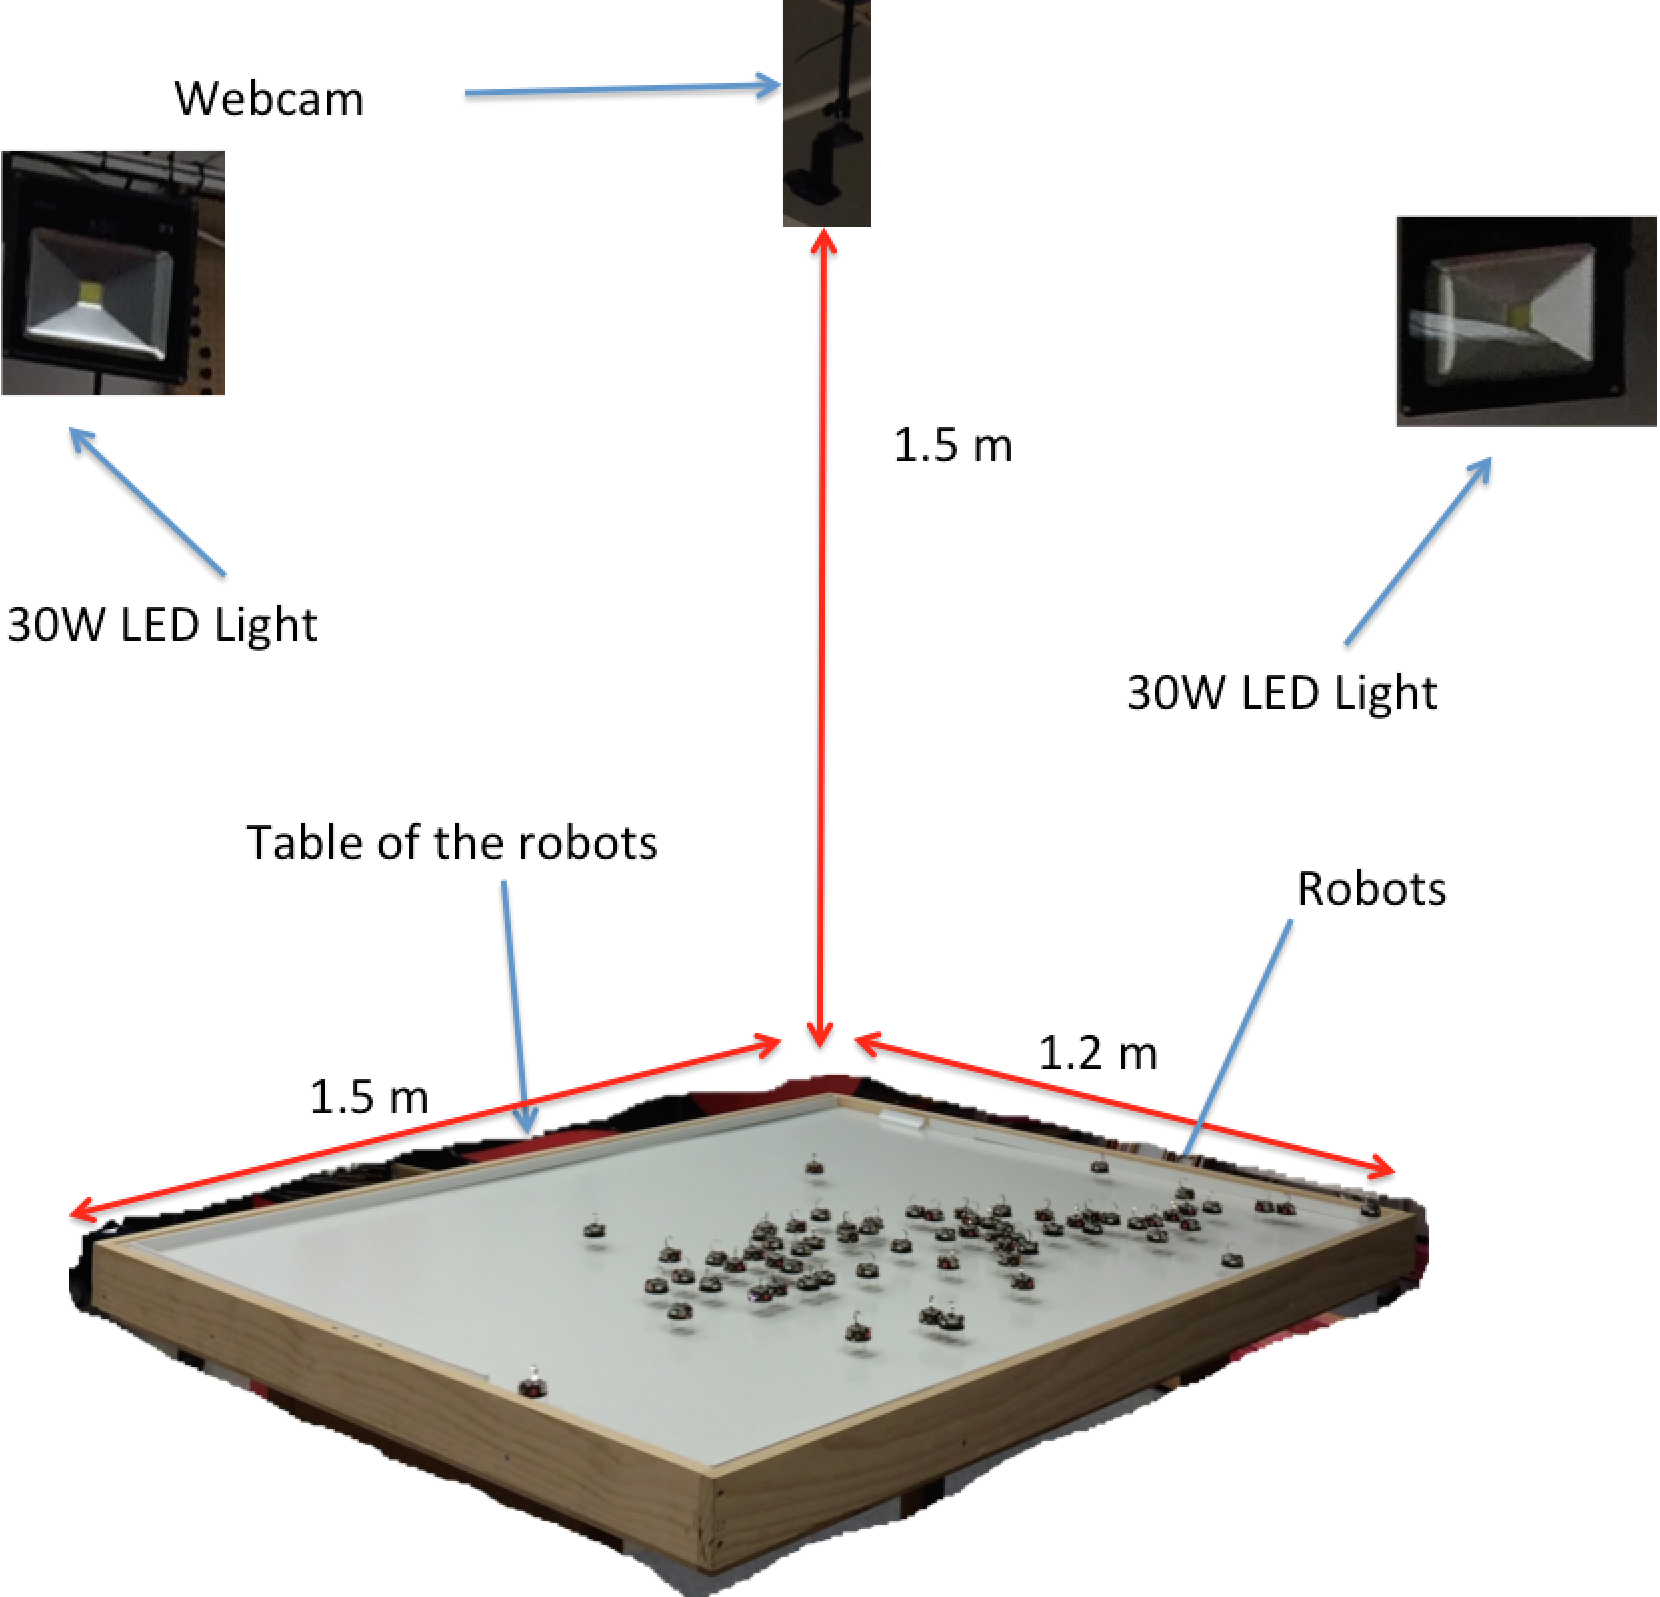
\includegraphics[width=.9\columnwidth]{SetUp.png}
\end{center}
\vspace{-1em}
\caption{\label{fig:setup}
Hardware platform:  table with 1.5$\times$1.2 m workspace, surrounded by eight remotely triggered 30W LED floodlights, with an overhead machine vision system.
}
\vspace{-1em}
\end{figure}





